\subsubsection{Komponen Pendukung: Konfigurasi dan Utilitas}

Seperti yang sudah dijelaskan sebelumnya, terdapat konfigurasi yang dapat mengatur sistem. Konfigurasi yang dapat diatur dapat dilihat pada gambar \ref{fig:config-spek}.

\begin{figure}[h]
    \centering
    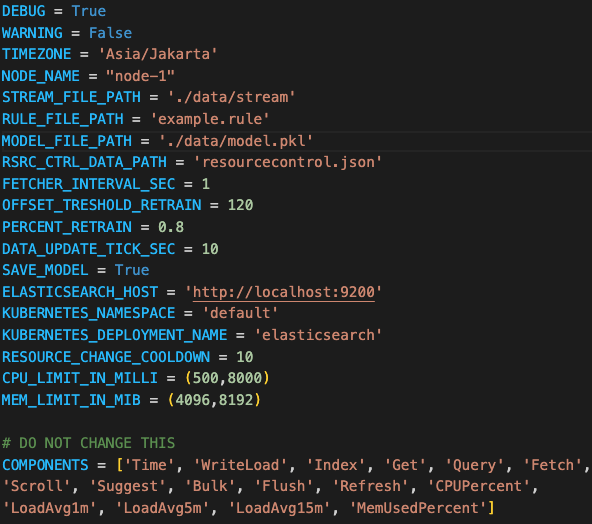
\includegraphics[width=0.8\textwidth]{chapter-4/config.png}
    \caption{Konfigurasi \textit{Flexible Control}}
    \label{fig:config-spek}
\end{figure}

Setiap konfigurasi tersebut mengatur perilaku dari sistem. Untuk setiap konfigurasinya, berikut adalah penjelasannya.

\begin{enumerate}
    \item \textbf{\textit{Debug}} dan \textbf{\textit{Warning}}
    
    Kedua \textit{flag} ini adalah untuk mematikan dan menyalakan pesan \textit{debug} dan \textit{warning}. Jika \textit{debug} dimatikan, maka program tidak akan mengirimkan pesan apapun selama berjalan.

    \item \textbf{\textit{Timezone}}
    
    Untuk mengubah zona waktu yang digunakan oleh pandas. Karena data yang didapatkan dari \textit{Elastic Search} adalah berupa unix time sehingga akan dibaca \textit{default} menjadi UTC saat dikonversi. Flag ini berfungsi untuk mengubah zona waktu yang digunakan oleh pandas.

    \item \textbf{\textit{Node Name}}, \textbf{\textit{Namespace}} dan \textbf{\textit{Deployment Name}}
    
    \textbf{\textit{Node Name}} adalah nama \textit{node} yang telah dikonfigurasi pada \textit{elastic search}. Nama harus sesuai karena \textbf{\textit{Metrics Fetcher}} akan mencari data untuk node dengan nama tersebut. Sedangkan, \textbf{\textit{Namespace}} dan \textbf{\textit{Deployment Name}} berkaitan dengan \textit{namespace} dan \textit{deployment Elasticsearch} dengan Kubernetes.

    \item \textbf{\textit{Elasticsearch Host}}
    
    \textit{Flag} ini berisikan target \textit{host} dari \textit{Elasticsearch}. Bertindak sebagai \textit{Base URL} untuk mengakses API \textit{Elastic Search}.

    \item \textbf{\textit{CPU Limit}} dan \textbf{\textit{Memory Limit}}
    
    Kedua limit ini digunakan untuk \textbf{\textit{Resource Controller}} mengubah alokasi sumber daya. \textit{Flag} ini berisikan \textit{tuple} dengan dua buah angka yang berguna sebagai batas bawah dan batas atas dari sumber daya bersangkutan. Satuan yang digunakan untuk prosesor adalah mili (m) sedangkan untuk memori adalah \textit{mebibyte} (MiB). Kedua batas ini bersifat inklusif.

    \item \textbf{\textit{File Path}}
    
    Seperti namanya, konfigurasi yang berkaitan dengan \textit{file path} berfungsi untuk mengatur tata letak file yang akan dibuat/dibaca oleh sistem.

    \item \textbf{\textit{Fetcher Interval}}, \textbf{\textit{Resource Change Cooldown}} dan \textbf{\textit{Data Update Tick Second}}
    
    \textbf{\textit{Fetcher Interval}} adalah interval komponen \textbf{\textit{Metrics Fetcher}} melakukan penarikan data. Lalu, \textbf{\textit{Resource Change Cooldown}} adalah waktu yang diperlukan oleh \textbf{\textit{Resource Controller}} untuk menunggu sebelum melakukan perubahan sumber daya. Terakhir, \textbf{\textit{Data Update Tick Second}} adalah interval yang digunakan oleh \textbf{\textit{Flexible Control}} untuk melakukan pembacaan data dari \textit{stream file}. \textbf{\textit{Data Update Tick Second}} harus lebih besar sama dengan \textbf{\textit{Fetcher Interval}} agar efisien. Satuan yang digunakan oleh ketiga \textit{flag} tersebut adalah detik.

    \item \textbf{\textit{Save Model}}
    
    \textit{Flag} ini berfungsi untuk mematikan penyimpanan model setiap kali model berubah. Jika \textit{flag} ini tidak dinyalakan, maka setiap kali sistem melakukan \textit{restart}, model prediksi akan diulang dari kosong.

    \item \textbf{\textit{Offset Treshold Retrain}} dan \textbf{\textit{Percent Retrain}}
    
    Dalam melakukan penambahan data, tidak setiap saat model akan di-\textit{retrain}. Saat tidak di-\textit{retrain}, model prediksi hanya melakukan update yang jauh lebih cepat namun tidak terlalu akurat. Terdapat sebuah angka yang akan menentukan kapan model harus di-\textit{retrain}. Hal ini diperlukan karena melakukan \textit{retrain} membutuhkan waktu yang lama terutama saat data sudah sangat besar. \textbf{\textit{Offset Treshold Retrain}} adalah angka yang menentukan kapan model harus di-\textit{retrain} berdasarkan jumlah data fixed. Sedangkan, \textbf{\textit{Percent Retrain}} adalah angka yang menentukan kapan model harus di-\textit{retrain} berdasarkan persentase jumlah data saat itu. Contohnya ketika saat ini data berukuran 100, dengan konfigurasi yang ada pada gambar \ref{fig:config-spek}, maka model akan di-\textit{retrain} ketika jumlah data sudah mencapai 200 atau 120+(80\% dari 100).
\end{enumerate}

Terdapat juga fungsi-fungsi utilitas yang akan membantu komponen-komponen yang telah dijelaskan sebelumnya, spesifikasi utilitas bisa dilihat pada gambar \ref{fig:util-spek}. Untuk setiap fungsinya, berikut adalah kegunaannya.

\begin{enumerate}
    \item \textbf{\textit{Save Model}}
    
    Fungsi ini akan menyimpan model yang telah dilatih ke dalam sebuah file. Digunakan kakas \textit{pickle} untuk melakukan hal ini.

    \item \textbf{\textit{Load Model}}
    
    Fungsi ini akan memuat model yang telah dilatih dari sebuah file. Digunakan kakas \textit{pickle} untuk melakukan hal ini.

    \item \textbf{\textit{Timings}}
    
    Fungsi adalah abstraksi untuk menghitung waktu eksekusi. Digunakan fungsi sebagai \textit{return value} agar lebih rapih ketika diperlukan banyak penghitungan waktu eksekusi.

    \item \textbf{\textit{Printd}}
    
    Fungsi ini hanyalah \textit{wrapper} dari fungsi \textit{print} pada Python untuk mengikuti aturan konfigurasi.

    \item \textbf{\textit{Read From File}}
    
    Fungsi ini digunakan untuk membaca \textit{stream file}. Fungsi ini digunakan oleh komponen \textbf{\textit{Adaptive Control}} untuk membaca secara periodik, mentranformasikan dan mengirimkan data ke \textbf{\textit{Predict Component Storage}}.

    \item \textbf{\textit{To Vector}}
    
    Fungsi ini adalah fungsi transformasi format JSON (\textit{Java Syntax Object Notation}) yang ditulis ke \textit{stream file} menjadi sebuah \textit{numpy array} yang akan digunakan untuk membuat \textit{pandas dataframe}.

    \item \textbf{\textit{Create Dataframe}}
    
    Seperti namanya, fungsi ini membuat dataframe dari data yang telah dibaca dari \textit{stream file} dan sudah ditransformasikan dengan fungsi \textbf{\textit{to vector}}.

    \item \textbf{\textit{Extract Number From String}}
    
    Fungsi ini memanfaatkan regex untuk mengambil angka dari sebuah string.
\end{enumerate}

\begin{figure}[h]
    \centering
    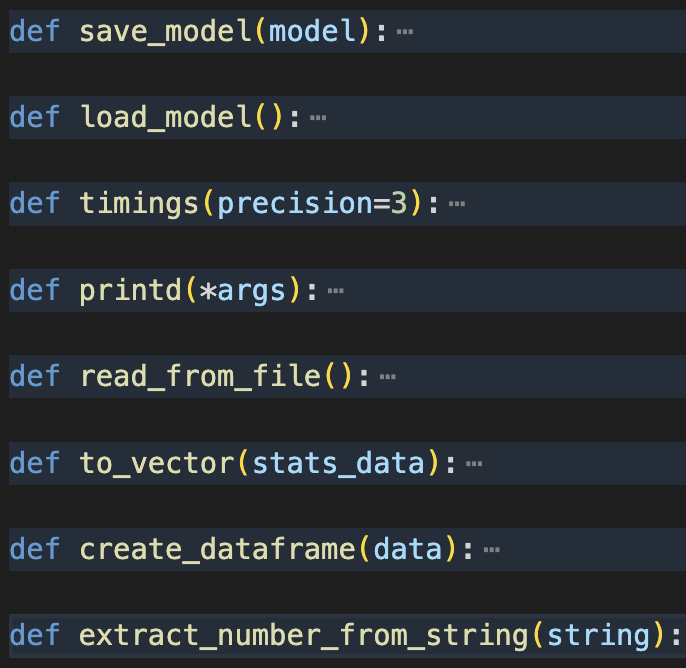
\includegraphics[width=0.6\textwidth]{chapter-4/utils.png}
    \caption{Spesifikasi Fungsi Utilitas Pendukung}
    \label{fig:util-spek}
\end{figure}